\chapter{\textit{Archipelago}}
Creating a hybrid game using PCG represents a challenge in both design and technical areas. First of all, the hybrid game genre that has been previously defined in this paper is a recent design space to explore for designers. Even though some experiments (like \textit{False Prophets} and \textit{STARS}) or games (like \textit{XCOM: The Board Game}) already exist, exploring this concept means raising many questions about how should the digital device be integrated, and what kind of play experience is enabled by the use of PCG. The best way to answer these questions is to make a comprehensive use of prototyping.

Some results from this experiment are more related to design choices that are not depending on PCG or the hybrid nature of the game. For that reason, the creation of \textit{Archipelago} is not to be thought as a universal answer to the use of PCG in hybrid games, but more as a way to point out, illustrate and explain the challenges that appeared while creating the game. In that sense, \textit{Archipelago} only provides answers to design and technical questions in a particular framework. However, since the game has been thought from the beginning as an experimental concept, it is expected that the answers provided by the different prototypes will transcend the project presented in this paper. This means that the results that will be presented here will contribute to the exploration of making hybrid games in various ways. The successful design choices must be situated in their particular context, and experienced game maker will recognize the patterns that worked. Using the same approach, the experimentations that did not provide the expected results will also be considered useful.

The following section will start describing the process of making \textit{Archipelago} by identifying the challenges that appeared when thinking about hybrid games using PCG. To follow, different aspects of the development will be described in order to clearly understand the purpose of \textit{Archipelago}. Each aspect of the game is analysed in the intention to provide results both on the design and technical aspects of its creation. 
\section{Brainstorming and Game Concept Choice}
Brainstorming over the concept of hybrid game was already a challenge in itself. Because of the experimental nature of the project and the time in which the game had to be created, it was decided to focus on the key challenges that were expected, and reveal new ones all along the process.
\subsection{Prior challenges}
In order to explore the use of PCG in tabletop games, the first step was to brainstorm around what PCG brings to the genre, and what were the pitfalls of such a combination. Based on the definition of hybrid games that was previously established and on the expectations of what PCG affords in games, the main ideas were pointed out (see appendix).
\begin{itemize}
\item A hybrid game is made of both digital and analogue components. The first challenge to keep in mind was that both types of components must be used for a good reason. In other words, the choice for the core mechanics must prove that the contribution of analogue components could not be simulated on a computer; the same perspective was adopted for the digital part of the game, which could not be replaced by any kind of analogue components.  
\item Another concern was to preserve the tabletop game experience, and not denature it because of hybridization. Therefore, the core concept of the game should stress out the particular element constituting such an experience. As previously stated, tabletop games cannot be reduced to the use of components, or the fact they are played on a table. The social dimension of tabletop games was the key element to stress out in order to make the analogue part of the game relevant.
\item Creating a hybrid game means comprehensively implementing a digital device to enhance the traditional game mechanics. \textit{Enhancing} does not mean creating \textit{better} mechanics. But based on the framework previously established, it was clear that the digital part of our game must "have a clear added value" (De Boer and Lamers, 2004, p.443)\cite{chap:aug}. This brings a new challenge which is tied to those above mentioned. The use of the digital component must bring something new to the tabletop game play experience.
\item The implementation of PCG must support the idea previously defined. Moreover, the concept of "replayability" (Smith et al., 2011, p.2)\cite{pdf:pcgbased} inherent to PCG-based game design must be illustrated by the game. The focus here was to make this concept visible by the players, who should understand that the game they are playing is flexible enough, so that they could replay the game without facing the same situations several times.
\item The concept of "player control" (both "direct" and "indirect") (Smith et al., 2011, p.2)\cite{pdf:pcgbased} over the procedurally generated content - linked to PCG-based game design - is also one that should be experimented thanks to hybrid games. It is one of the enhancement that was hoped to be achieved and tested throughout the project. It has been previously stated that player control is an interesting contribution of PCG-based game design, as it triggers an uncertainty related to a sufficiently varied creation of content. The players should feel that they have a certain control over the content generation, but still be surprised by unexpected outcomes.
\item This leads to "adaptability" (Smith et al., 2011, p.2). The adaptation the content to the player's actions in the game would be one of the crucial aspect of the experiment, because it shows one aspect that is hard to recreate in tabletop games without the use of computing (though certainly not impossible). However, by using a large number of parameters to feed the PCG algorithm, the content generation would provide a variety that is in this case definitely impossible to reproduce with only analogue components.
\item Finally and to stress out the core tabletop gameplay, it was necessary to be cautious about how intrusive the application would be in the game. One of the challenge while designing the game would be to provide enough information to the digital device, so that a sufficiently varied content could be generated without requesting too many inputs from the players. More generally, avoiding \textit{algorithm specific inputs} that go directly as parameters to the algorithm in order to customize it to the next state of generation was necessary. Therefore, they should be well hidden  behind the game mechanics.
\end{itemize}
Those challenges were the main ones that the project should cover. To do so first required to find a game concept based on core mechanics that would allow the exploration of those challenges.
\subsection{Concept meeting the challenges}
Based on the principles previously stated and on the related design pattern theory, a first game concept based on a core loop had to be found. The patterns had to support each other, put the players in front of dilemmas and be blended in one core loop on which the whole gameplay would be based on. 
\subsubsection{PCG-based design pattern}
The first design pattern that was considered (extracted from PCG-based games) was the \textit{Node exploration}. The player would need to explore nodes displayed on a map towards a final destination (see figure \ref{fig:map}). Examples of such mechanic can be found in \textit{FTL: Faster Than Light} \cite{game:ftl} or \textit{Out There} (Mi-Clos Studio, 2014)\cite{game:outthere} - which both inspired the creation of Archipelago. The players would have to travel or select the nodes one by one on the digital device supporting  \textit{Archipelago}'s gameplay, and progress thanks to the outcomes procedurally generated in the nodes. This pattern had several benefits, and also several implications. 

First of all, the node's content varies depending on the game, but is often based on a risk versus reward concept. The player has to foresee the potential reward that an event can provide, and balance it with the necessary risk to take in order to access it. The crucial part of this idea is to be found in the \textit{necessity} of the risk, and the \textit{possibility} of getting a reward. 

The outcomes depend on the player's choices at each node. Generally, the difficulty of the choice that the players have to make in PCG-based games enables the very specific pleasure - and sometimes frustration - of randomness. However, this kind of risk versus reward play experience is very frequently used in tabletop games (often reproduced with a dice roll). For this reason, another value should be added to this pattern, thanks to the use of PCG to create the nodes and their content. This would be included in the scope of several prototypes.

Also, this pattern naturally fits into a gameplay loop. It is a mandatory action that can overthrow a situation if the risk taken by the player is too big - in the case the player is unprepared, or if the risk was not realistically estimated. Finally mechanics based on this pattern using PCG are challenging to design because of the many possibilities that the players can be confronted to. 
\begin{figure}[h]
    \centering
    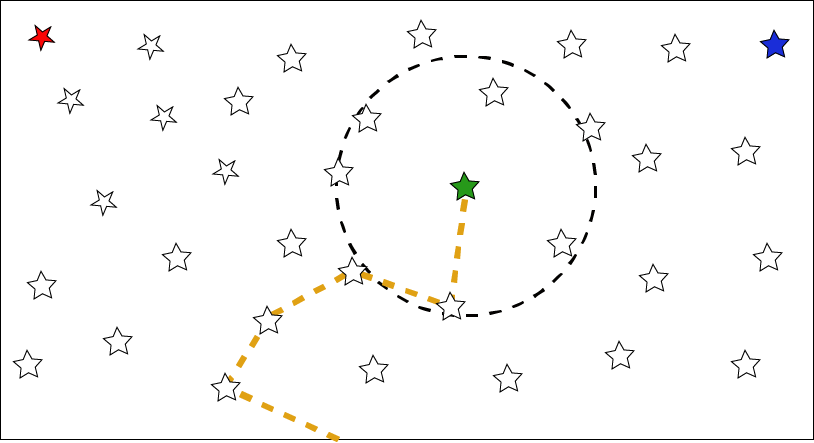
\includegraphics[scale=0.25]{Images/Map.png}
    \caption{First map mock-up used to communicate the basic concept to the team. The green node represents the position of the player, and the red and blue stars are nodes that need to be visited. The circle around the player limits the nodes that can be reached in one move, and the yellow line shows the already visited nodes.}
    \label{fig:map}
\end{figure}
\subsubsection{Board Game mechanic}
The \textit{Base Management} pattern is the next one that was chosen to create the analogue part of \textit{Archipelago}. The term \textit{base} refers to the central part of the game, that the players would use to travel from one node to the other. This pattern is closer to tabletop game mechanics, where the players uses the different resources available to progress through the game. As an example, the game \textit{Agricola} (Rosenberg, 2007) \cite{game:agri} illustrates this mechanic in various ways: the players need to improve their resources collecting capacity in order to manage their farm and their family. This create a progression based on the player's ability to manage resources correctly in order to produce more resources during the later turns in the game.

In \textit{Archipelago}, the resources would have different uses and origins. On the same principle, the various ways in which the base could be upgraded would provide a variety of gameplays and strategies, thus enforcing the "replayability" of the game.

\begin{figure}[h]
    \centering
    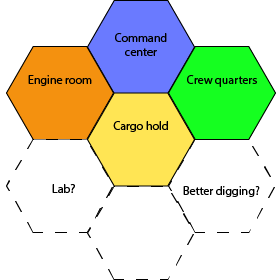
\includegraphics[scale=0.5]{Images/Base.png}
    \caption{Early mock-up describing the tiled structure of the base. Each hexagon represents an upgrade of the base.}
    \label{fig:base}
\end{figure}
\subsubsection{A collaborative board game}
By combining those two main design patterns, \textit{Archipelago} would merge mechanics specific to PCG-based with mechanics that could well be based on a game board, although not specific to the tabletop genre. An additional element from the tabletop game definition was then required to make the physicality of the game a crucial aspect of the game, and justify its \textit{hybrid game} denomination.

To make a successful combination of board game mechanic based on tiles and exploration of locations based on PCG, it was decided that \textit{Archipelago} would be a collaborative game. One single base would be shared by all the players, who would have different roles and specialization. This approach can be found in variety of games (both tabletop and digital) and one example has already been described when presenting the playthrough of \textit{XCOM: The Board Game}. Designing the game as a collaborative board game would emphasize the social dimension of tabletop games. This is one of the thing that makes the board irreplaceable in the case of Archipelago. The board would provide an interface around which they can gather and plan the management of the base and the allocation of the necessary resources. Discussions occurring during the exploration of the nodes would be influenced by the fact that the players would have authority in their area of expertise. This expertise would enable a feeling of importance, and mechanics supporting that feeling would need to be explored as well.

The collaboration would also enhance the PCG-based mechanics of the game in an original way. Indeed, games using this mechanic leave their player alone when evaluating the risk of performing or not an action. This time, the players would need to take the decisions together, even if one of the player is specialized. This different approach would also bring another kind of flavour to hybrid games, and it was hoped that the discussion that would take place before performing the events would provide an enjoyable experience.
\begin{figure}[h]
    \centering
    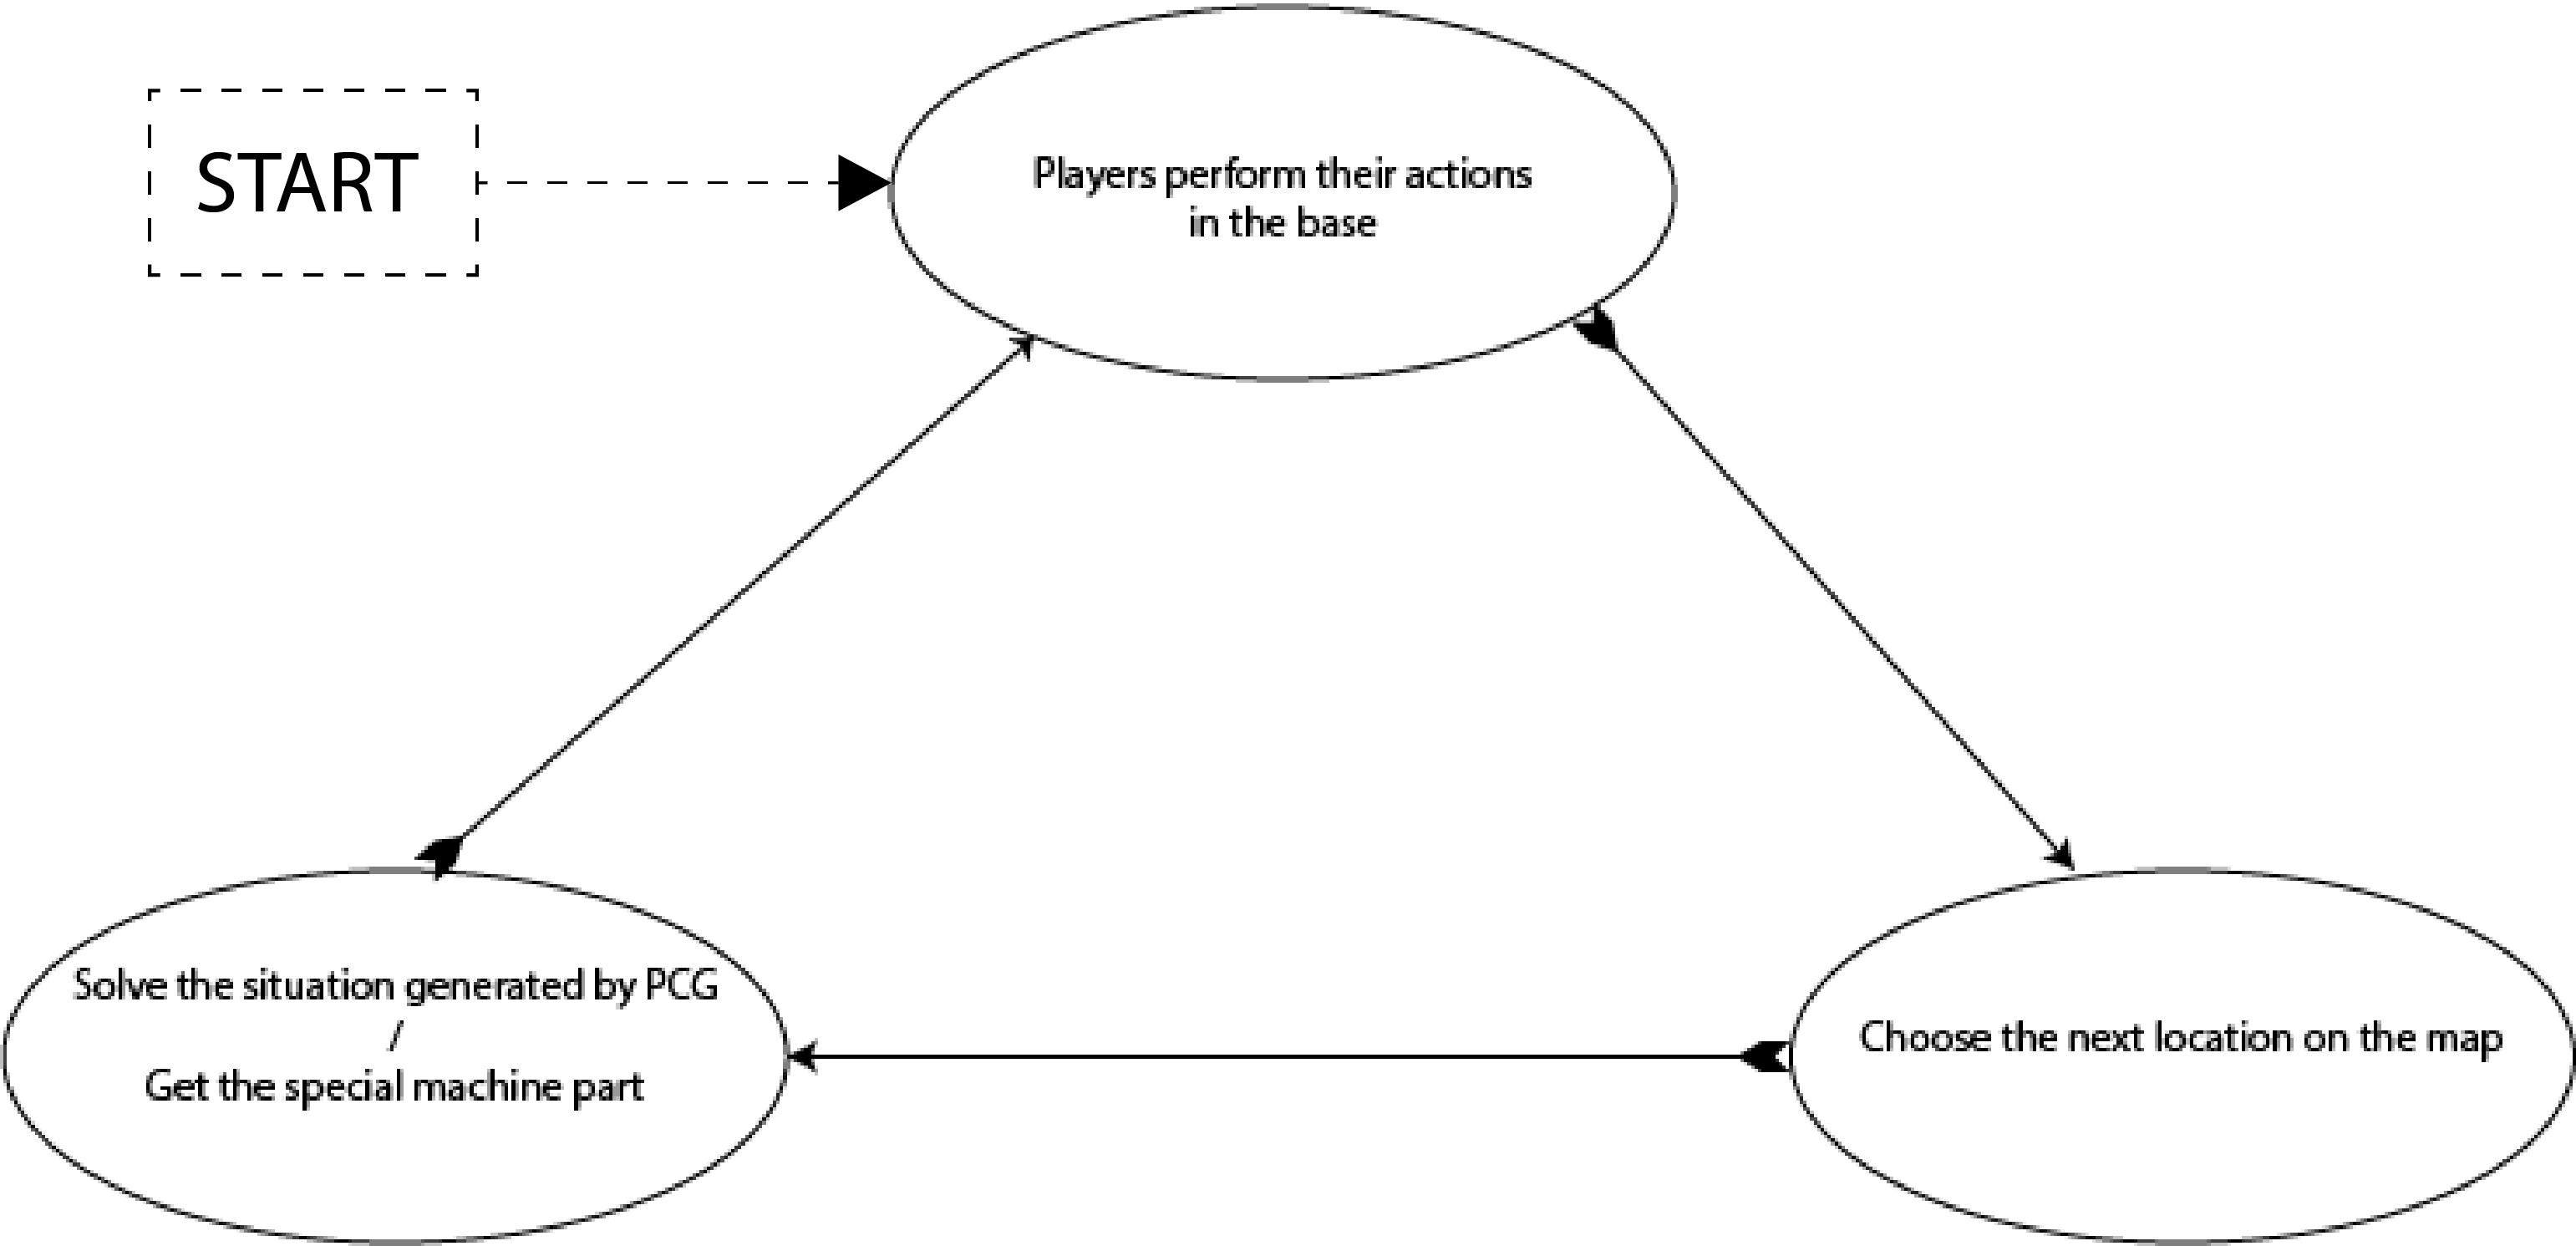
\includegraphics[scale=0.5]{Images/Core loop.png}
    \caption{A visual representation of the core loop, composed by the three different steps composing one turn.}
    \label{fig:loop}
\end{figure}
The combination of those patterns was the base of the core loop (see figure \ref{fig:loop}). The players would have to collaborate managing their base using the resources found during the event exploration. The events would be procedurally generated and only occur on the digital device. This intricate the analogue part of the game with its digital part, as the strategy chosen by the players during the management phase of the game would condition the choices made during the exploration of the events.

\section{Designing \textit{Archipelago}}
Building over an abstract game concept requires another brainstorm session to explore the possibilities offered by such mechanic, and exploit the digital component using PCG. The inspirations found after the brainstorm session gave several directions to explore potential hybrid game specific experiences.
\subsection{Hybrid game system}
Setting
Management system
Resources
Player Specialization
Risk/Reward
Infinite number of cards (events)
Event "memory"
Special events
UX (App/Board)
\subsection{The role of the digital part}
Mainly, the function of the application is to contain all the information regarding events, movement, factions and overall the data available within the game. The application is the only connection the players will have to what is supposed to happen in the game, as without it, the game would just be an empty board with pieces that would have no purpose. 
When playing the Archipelago, the digital part of the game, the app, will provide the players with a layout of the world, i.e. the map with all its islands, and it will contain all methods of receiving rewards as well as receiving penalties for executed events. It determines which resource the players will receive, what the "story" is, in terms of flavour presented, and it contains the factions and the players standing with each of them.
The events in the app, are made to be like cards that the board game would have, if there was no app. But by having the digital computing and memory, the diversity of these events are much greater and there is no need for a huge pile of cards and expansion packs to generate different and diverse events. The app is in full control over what the players get and what is taken away from them, and given that there is now memory in place, the possibility to create new content based on previous events is there. Another part that the application plays in the entirety of the game, is that it controls when effects take place. If there has been an event with a specific outcome, it is then the system that controls if there should be consequences based on those outcomes. If there was no digital application in place, there would have to be a large amount of cards and pieces in the board game, along with very specific rules and combination guides, for the players to sufficiently be able to piece together new events and outcomes. So the biggest purpose of the app, as implemented in this solution, is to have complete control over all actions, story, events and outcomes and be able to present them to the players without using much time, which the players would do if they had to combine their own "gameplay".

\section{The Game - One play session}
In this section of the paper, we will go through a full play session of the game, that is all the different stages that occur in a game session, and explain the actions that happen along the different phases of the game.
The game session presented will be a fictional one, and the game itself will not necessarily be a complete one in terms of going through all the islands that would be represented on the application at runtime, but rather it will explain every step along the way, and go through all the main parts of a complete game session.

\subsection{Setup}

When starting the game, the first thing that will happen, is to set up the board. The board will be placed on the surface area that the players are using, i.e. a table, and the starting conditions, like the initial resources the players have, will be distributed onto the board. Next step is to assign the player tokens to the respective players. Each player will have their own color on their own "crew tokens" and the color itself is arbitrary, and has no relevant meaning to the game itself, rather than making it easier for the players to know which one is theirs.
When the assigning of the player tokens have been done, and the board has been placed, if the game is played by new players, the next step will be to read through the rules of the game, and to have one of the players read out loud and explain the different phases and the possible actions that can be done, along with the costs and rewards of said actions. If this is not done during the start-up of the game, it can also be done at runtime, as there is no set timer within the app, and the players can take the time they need and reference the rules when needed.
After all this initial setup is complete, the only remaining thing to do, is to start up the application part of the game, and be presented with the map that the game session will explore.

\subsection{The Board}
When starting the game and placing the board, the initial pieces the players have available are 2 player tokens, or crew tokens, for each player in the game, along with 4 building materials and 1 alchemy point. The castle itself will start off with 3 crystal pieces, which power the castle, and these 3 pieces are enough to start the players off with their castle at tier 1. In order to get to tier 2, the players will need to acquire another crystal piece.


- Starting pieces, etc.

\subsection{The App}
As the application is started, the players are presented with the layout of the map. In the center you will find the castle, as is being represented by the physical board on the table. To move around in the world, all that needs to be done, is to click on an island that is within the circle around the castle, which indicates the travel distance possible for the castle each turn. Once an island is clicked on, a travel confirmation dialogue box will appear, and the players will have to confirm that they do indeed wish to travel there. As the castle reaches the selected island, the events begin. 

- Starting the game and moving around the world

\subsection{Phase 1 - Castle Management}
Before the players have to travel around the world within the app, they have the first phase on the board. This phase is called the management phase. 
In this management phase, the players can upgrade, repair and expand upon their castle.
There is no limit for how much they can do, other than what the players themselves have the resources for. If they want to build a new room, this can be done. However, the cost of doing so is 2 building materials, and a player will have to assign one of their crew tokens to the building task, and that means that that token can not be used in the upcoming event phase this round.\\
If there already exist one or more rooms in the castle, the players can choose to upgrade it to the next level, though they still need to have the required resources. To upgrade a room from tier 1 to tier 2, you will need 2 building materials in order to build the 2nd room, and you will need 1 alchemy point for each room that is being combined, so in this case it would be 2 - one for the old and one for the new. Again, this will require a player to temporarily set a crew inactive, as it has to build the room.\\

Before heading out into the world map, the players can choose to assign their player tokens to the rooms they have built. If they would like to receive more building materials on the upcoming event, they would have to put at least one crew token on the mining room that they would have built. Likewise for alchemy points, they would have to place a crew token on the alchemy room. 

When travelling out into the world, the players would need at least 1 available crew token, as the minimum cost of an event option is to send a crew. Otherwise, they would technically not be able to "explore" the island, as none would be out exploring.


- Building rooms\\
- Assigning people to rooms\\
- 

\subsection{Phase 2 - Exploring the World}
When the first phase is over, and all the crew tokens have been assigned, the next phase is to explore the world.
As mentioned before, the first thing the players have to do in the world map, is to click on the reachable island they want to travel to. Once they have accepted to travel there, and have reached the location, the players will have to select an area, or location, that they would like to explore.\\
Each area are connected to a type of resource, either it is a gathering area which will mainly yield building materials, or it is the research area which will yield mainly alchemy points.
The players talk amongst themselves which one they would like to explore, and will have to choose based on what their current needs are. If they are low on building materials and want to build a new room in the next management phase, they might want to go for the gathering location. If they want to upgrade a room next turn, they might want to go for a research location.\\
Once a location has been selected, the players will be presented with the event.
The player who is currently controlling the application reads out the event along with the possible options.
It is now up to the players to talk amongst themselves to figure out which option they would like to pick. The first option is usually just sending a member of the crew down to complete the event, but there can be other options as well. Say the 2nd option is to send a crew along with an alchemy point, and the third option is to send a crew, 1 alchemy point and have a healer. 
If the 1st option is selected, the players will have to decide which player uses their token, as the outcome might be that it dies.
If the 2nd option is selected, the same question goes: Who sends their token? It might also be the case that they do not have the required alchemy point to spend, in which case they cannot complete that option.
For the 3rd option, the players will need to have the healing room specialized. If they do so, they will have to decide whether or not it is worth the risk of selection that option, or if they should chance it on something else.\\
After the players have reached their conclusion and selected their option, the application will present them with the resulting outcomes of the event. It might be that they have lost a player token, gained one, a room has been destroyed, or simply that they got some resources. The outcomes vary.
When the players have received their rewards and applied the results to the board, the game goes on to the next phase.


- Travel to an island\\
- Picking a location - gathering/research\\
- The event occurs\\
	- Talking amongst the players\\
	- Selecting a viable option\\
	- Assigning player tokens + resources\\
	- Completing the Event and apply the results to the board\\

\subsection{Clean-up and Reset}

When returning from an event, all the pieces that were used the previous round, i.e. the crew tokens used for construction, the tokens assigned to the rooms, and the tokens used in the events, are returned to the players, and the board is cleaned up.
If an event yielded too much resources so that the cargo hold of the castle would be overfilled, it is up to the players to discuss which they would like to keep, and which to discard, before going back to phase 1 - management.

When this is done, the game repeats as described above with phase 1 and 2 and back again.

\subsection{Special Event Occurs}

Somewhere along the game, the players will most likely encounter the "special events". There are as of right now, two types of special events.\\
The first type is the fighting event. When this event occurs, the players will be presented with a scenario where two of the factions within the game, are fighting each other. It is then up to the players to decide whether they want to leave them alone, or if they would like to assist them. If they want to assist them, they have to choose their side. If the players are already friendly with one of the factions, they might want to assist that faction again. This choice is completely up to the players.\\
The other event type is memory based. It is an event that is based on previous events that the players have completed. If they can remember it, all the better. Either ways, the event is special in that is based on previous data. If the players visited an island controlled by the Highbournes, and they used some special healing on one of the options, then the special event could say something like "The highbournes saw you at the island, and want to learn how to use your healing magic". It is then up to the players to decide whether or not they want to help them, or not. Keeping in mind that their current standing with the faction will influence the outcome of whatever option they choose. 

\subsection{Reaching the end - Winning condition}
At one specific point on the map, there is a goal island. This island is the one the arrow is pointing towards, and is the one that the players are supposed to head towards in order to complete the game, and win.
If the players are able to reach this island, the game is over. The players will be presented with an ending screen in the app, and then they can choose to start a new game if they so choose. 

\subsection{Losing the game - Losing conditions}
There are a number of different ways to lose the game. Since it is a collaborative game, if one of the players manages to get all his or her crew tokens killed, the game is over. Every player must have at least one crew token, in order for the game to still be in play.
Should the castle run out of crystal charges, the game will be over as well, as this would mean that the castle would be stuck floating in space and not be able to move.




\section{Development Structure (Technical)}
This part of the paper will go into more detail on how the development of the project went as seen from a more technical aspect. This includes making prototypes, the way to go from communicating with a designer to implementing a solution, and lastly problem solving along the way.
\subsection{From design to implementation}
When working as a developer, you also work closely with the designer. What we did during our development period, was to get the wants and needs from the designer, and try to implement it into prototypes for overlook and feedback. 
If things needed to be changed, added or removed, the team would go through in general terms what needed to be done, and then the requested adjustments would be made to the prototypes.

In the next part of this section, we will go into more detail on how the prototyping would take place, how the communication between programmers and developer happened, and what changes were made over time during the period of development.

\subsection{Prototyping (Application)}
Right from the start, it was important to quickly produce smaller prototypes so that we could get an idea of how to continue, and to test the implementations that were made. The first part of the project is to set up the app and have a starting point that you can build on. In our case, this meant an initial screen with a simple UI that could be added to, moved around and overall that could display text and data. On top of that, the backbone of the system would be to have different data classes that could contain the various sorts of information that would be needed.

\begin{center}
\textbf{Prototype 1:}
A simple UI with text boxes, buttons and a simple data manager that contains the initial values.
\end{center}
Going onwards, designer and programmers alike, would come with inputs to set the foundation for which data types would be needed in order to produce the desired results.
It was decided early on that there would be events that the players could interact with, and that these events would have board pieces and flavour text associated with them. The basic layout for the \textit{flow} of the game is then set, with the idea that there would be a main world scene where all the destinations would be displayed, and each of these destinations would have their own scene where the locations possible would be shown.

\begin{center}
\textbf{Prototype 2:}
Now the application has a main world screen with a multitude of destinations would be displayed in the form of simple spheres that can be clicked. When clicked, the destination scene would be shown, which contains the simple representation of locations, also in the form of spheres.
The map layout is generated by using an L-system algorithm (see \textit{PCG - Generating the content}).
\end{center}
At this point, the need to link the application with the board game occurs. A player object is needed within the application, and it needs to be able to move around the world space. Also the initial event structure is taking form, which means there is a need for the data to be constructed along with some dummy flavour to be shown on the screen.

\begin{center}
\textbf{Prototype 3:}
Introducing the player object, the event class and XML files with the initial flavour texts. 
\end{center}
The events and the data contained is rather simple at this point. An event is mostly consisting of a simple description, a set of premade options, and one or two outcomes that are also premade. So a few events were made by selecting different descriptions, along with randomly selected options and an outcome for each option.\\\\
With the backbone in place for creating "varying" events, the next logical step, is to start coming up with the algorithm for how the events should be constructed and generated (the actual algorithm for how it works can be seen in the "Events" section later in this document).

\begin{center}
\textbf{Prototype 4:}
With a better working event generation system, the next prototype is made with a wider array of option possibilities, along with more outcomes.
\end{center}
So now the basis for the events are in place. The next part of the application, will be to have a more diverse collection of flavour texts.
This meant that we would have to come up with how the flavour text should be combined (see how in the \textit{Flavour of the Events} and in the \textit{Discussion} section later in this document) and create an algorithm for doing so. 

\begin{center}
\textbf{Prototype 5:}
Event generation is in place along with flavour-combining algorithm.
Everything seems to be working as intended, with the exception of some bugs here and there. But the overall main event system that allows the first play through of the game, is now in place.
\end{center}
After going through some plays of the game, and as more design decisions are made, more functionalities have to be implemented. The next step in the prototyping cycle would be to get a faction system going. What this would mean on top of the actual faction system itself, is that there would have to be changes made to the flavour combinations, as the resulting texts would now have to include the factions. Furthermore, there would have to be special events and rewards/results from events, that would affect the reputation the players would get with the respective factions.

\begin{center}
\textbf{Prototype 6:}
The faction system is implemented, along with a set of special events and outcomes that can be triggered via the regular event system. Now an event can have a 3rd option, which will have the chance to trigger the special events. There are 2 types of special events implemented, the first is a faction-war event, which would let the players choose sides between factions, the second type is the big ones that are based on previous experiences and encounters that the players have had within the game. When the 2nd type of special events are selected, it will take various data from the event that triggered it and use those in special combinations to give the players the experience of \textit{history} and \textit{consequence}.
\end{center}
By now, the application has most all of the structure and algorithmic computation and generation needed to make the game a complete experience.
The remaining tasks to be solved, is implementing better visuals, icons and signifiers. Scaling the elements to fit the tablet on which it will be played, and making sure there are as little bugs as possible.

\begin{center}
\textbf{Prototype 7 - Archipelago is born}
The final product is ready. No more coding and algorithmic calculations are needed. From this point in, polish is the keyword. Optimizing the feel of the application, making sure everything runs smoothly and looks good, and having as many flavour text pieces as possible for every element, so that the game will be as diverse as possible.
\end{center}

\subsection{Problem solving}
One of the biggest concerns in terms of being able to present the game with "feel" to the players, was to come up with a way of generating the flavour text. The design choice made was that it would be combined by lesser blocks of text that would be combined into one complete sentence that would display the entirety of the flavour. The way to go about this, was to create dummy data and reverse engineer that into a combination system. First you would create a complete flavour text that would be served as an example. This text would contain a combination the elements that would be wanted in the actual implemented solution; Location types, island names, factions, resources, outcomes, etc.

To exemplify, we will use the dummy flavour "As you arrive at Endriath, you see an old village in the distance. The village seems to have markings that resemble those used by the Highbournes".

The next step would be to reverse engineer this dummy text into blocks of strings that could be combined to reconstruct the original text. So in the start, there is a segment that says "As you arrive at ...". This part would act as an introduction for the island. Next you have the actual name of the island, which is already available in the application. After that there is a smaller part that gives the players insight into what \textit{is} on the island. This segment, however, is split up into 3 pieces; first - "you see ", then "an old village" which is the location type, also available within the application, and lastly " in the distance". After this, the flavour goes on to say something about the location that you are currently at. "The village", again, is available from the application, "seems to have markings that resemble those used by the" - extra flavour made to build mood and a sensation of lore or story, then at the very end is the "Highbournes" which is the faction name of one of the factions saved within the application.

This way of reverse engineering a piece of text leaves us with the pieces: Introduction, Island name, Location introduction, Location type, Location exit, Location Type(again), Mood flavour and Faction name.

After all these pieces has been discovered, the next step is validation. This is done by simply making a set of paper prototypes for each of the pieces, each having a few different possibilities, and then trying to combine them in the same fashion as discovered by the reverse engineering. 

When this all succeeds, the method of combination is discovered, and is ready to be implemented into code. Then, when it is all implemented, all that needs to be done, is to create a variety of flavours for each of the blocks and the rest will be done by the program.

\subsection{App structure}
This section details the different scenes which are in the app and their function. 
Each of the scenes will be explained in detail in the following sections.
The scenes included in the app and the change between the scenes are detailed in figure \ref{fig:appState}.

\begin{figure}[h]
    \centering
    \includegraphics[scale=0.5]{Images/StateDiagram.png}
    \caption{The overview of the scenes in the application and their linkage. The diagram shows each of the actions which change to other scenes.}
    \label{fig:appState}
\end{figure}

\subsubsection{StartScene}
As the game is started, you immediately enter the start screen. This is a simple scene containing only the button that says "Start Game". The purpose behind this scene is to let the users be able to chose when they want to start the game, so that they are not necessarily overpowered by the rules of the game (board game part) and the visuals of the app itself when started.

Furthermore, as this scene is loaded, the preliminaries to the world generation and the loading of required data from XML files is handled. This minor loading, takes some of the load of the rest of the program, giving an overall smoother experience.

As soon as the "Start Game" button is clicked, the app will generate the contents of the world, and present it to the user within the next scene, which is the WorldScene.

\subsubsection{WorldScene}
This is the main layout of the world. It contains all the locations that the players can travel to, and shows them where they are, where they have been, and where they have to go.
When you first see this part of the program, you will notice that it has floating islands with circles around it, as well as a flying castle. The castle is the piece the players control, and it is what the board is representing in the physical part of the game.
At first glance, you might not see all of the map and all the different islands you can travel to, but by simply zooming out, the players are able to get a better view of the entire map layout, and from there, they can plan their chosen way. There is also a little arrow in the lower right corner of the screen, which always will point towards the goal-island. 
The layout of the WordScene can be seen in figure \ref{fig:worldSc}.

\begin{figure}[h]
    \centering
    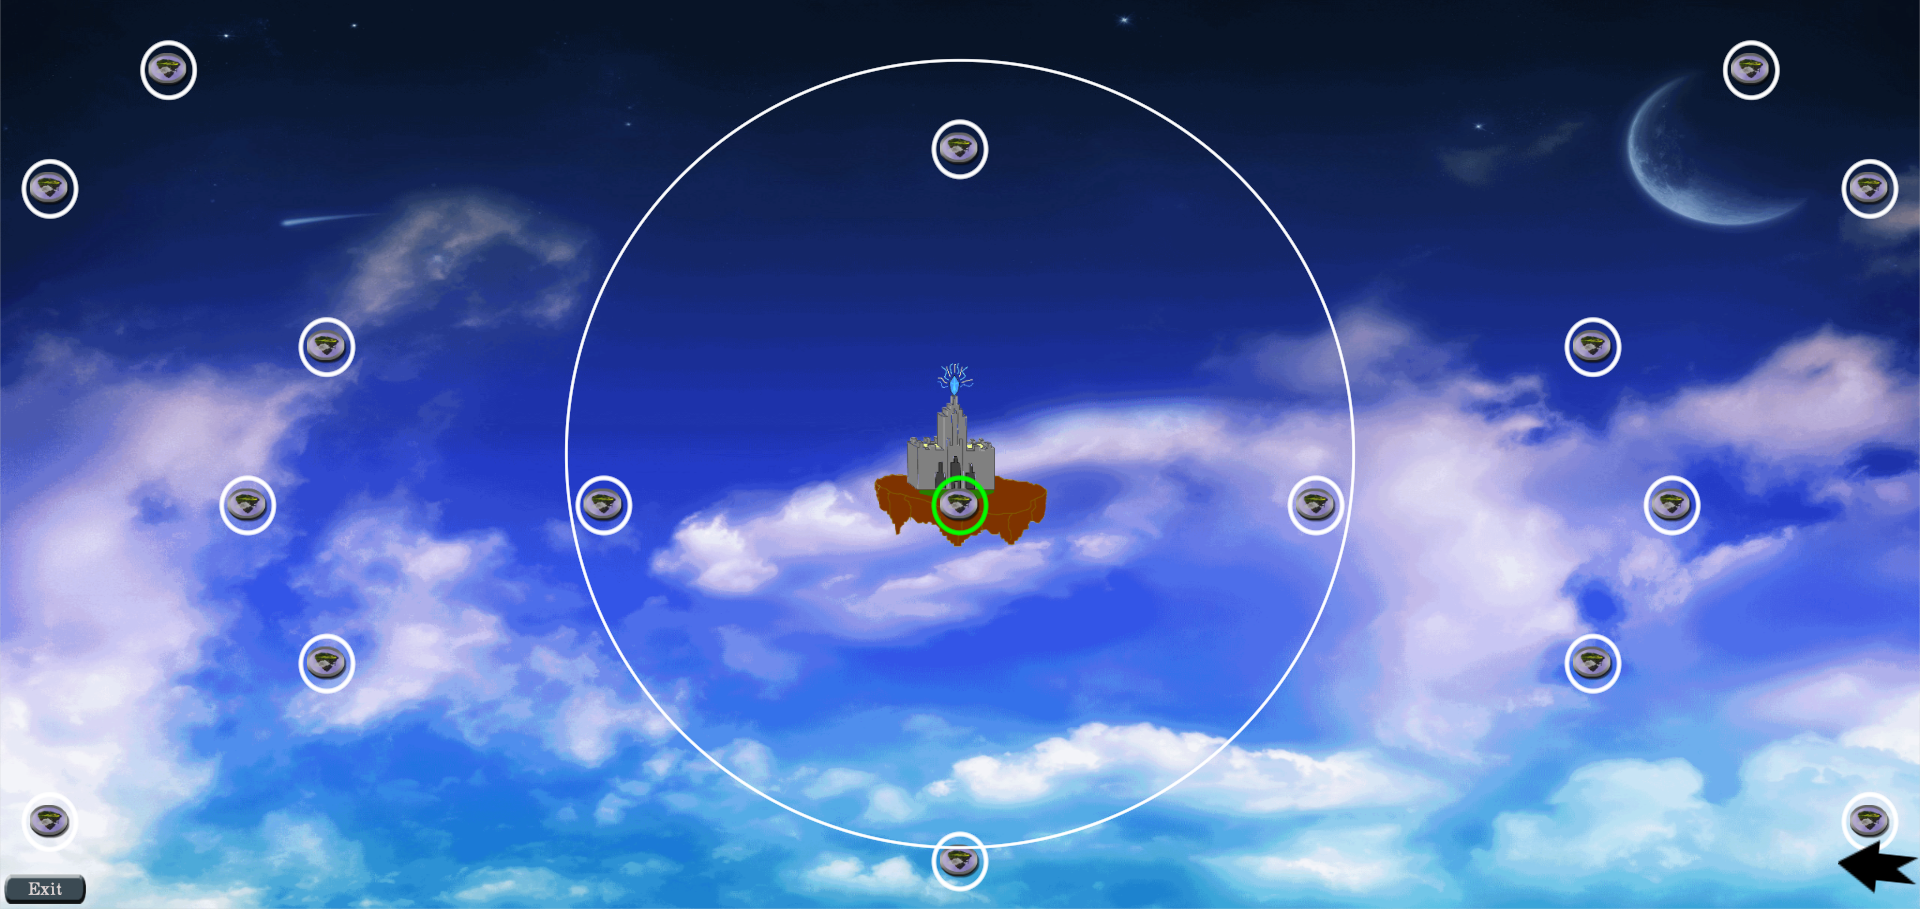
\includegraphics[scale=0.3]{Images/WorldScene.png}
    \caption{The WorldScene as seen on the PC version of the App. In the center the player token is represented as a floating castle. Also seen in the center is the green node, denoted as the starting node. In the lower right corner is the arrow pointing towards the goal node. The outer white circle indicates the maximum travelling distance of the players.}
    \label{fig:worldSc}
\end{figure}

Centered around the castle that the players control, you will find a large white circle. This circle is indicating the range that the castle can travel in one turn of the game. Any islands that are within this circle, are available to be travelled to.

When travelling from one island to another, the circle around the island you arrived at will change color (from the initial white color). This signifies to the players that they have already been to that island and therefore do not necessarily have to go back to that place again unless they choose to do so.
When you click an island on the map, you will be faced with a pop-up box. This box is containing the name of the island, and a piece of text that somewhat describes it; flavour text. The box then has 2 buttons, or choices, either "exit" or "travel". If you exit, the box is closed, and you are free to choose another island to travel to. If you click travel, however, your castle will be moved towards that chosen island and stop once it reaches it. 
Once the castle has reached the island and the collider on the object is triggered, the app will move on to the NodeScene, where the island that you travelled to will be represented.

\subsubsection{NodeScene}
\label{sec:nodeScene}
The NodeScene is probably best known as the "island scene" or "event scene", because 
this is the scene where all the events take place, and it is the main place where the players will have to interact with each other in order to choose their wanted event. 
To briefly describe the looks of the Scene, it has a background representation of an island, and on that island, it has image representations of the locations that the players will be able to travel to. On top of that, every Island (from the WorldScene) has a faction affiliated with it. What this does, is to allow the player to instinctively know whether or not an event can have a positive outcome and if it has a higher chance of success, based on the current standing the players have with that faction.
Once an area of the island has been clicked, let's say they chose a mine, a confirm box will be shown where the player will have to confirm that this is the area they want to explore. 
There are 2 main types of events; Research and Gathering events. Research events usually yield more alchemy points, whereas the gathering event has their basis in building materials.
After the confirmation, a new box will appear, where the event flavour text is presented along with either 2 or 3 options. Each option contains between 1 to 3 board pieces that will be utilized in order to complete the event. I.e. send 1 castle crew along with 1 alchemy point for a potion, etc. As soon as an option is selected, the event is concluded and the players are presented with the results; Success, Failure or Neutral. Each of these outcome types has rewards or penalties associated with them.
The last box that will appear in this scene is the result box where the players then have to click "return to world", and are then taken back to the WorldScene. 

\subsubsection{ScoreScene}
Upon reaching the final island in the WorldScene, the one island with the blue circle around it and that the arrow, that was mentioned earlier, is pointing towards, the game ends. What happens then is that all the data is cleared from the app, the WorldScene shifts to the ScoreScene, and the players are presented with an end text that basically tells them that they reached the goal. This scene also includes a button that takes the players back to the StartScene where they can play another game if they so choose.

\subsubsection{Island Nodes and Location Nodes}
All over the world map, there are placed a lot of islands. These islands are the places that the players can travel to, and they are represented by a picture of an island that floats, along with a signifier-circle that tells the players whether or not they have already explored it. Inside each of these islands, there are a bigger image that represents the island itself, and on that island, or next to it if there is a "floating rock formation", are smaller images of the available locations that the players can explore. 

All of these nodes, islands and locations alike, are what gives out the events to the players, and they are what causes the story and feel of the game by containing all the events, their flavour, rewards and owners. All of this information is going to be presented to the players at their command, and this means that they must have some way of interacting with them. This is done via use of the UI elements (see the "UI elements" section), and in particular the buttons and images.

\subsubsection{Buttons and Raycasting on images}
As explained in the section above, the players main source of interaction is via the use of buttons and images. The buttons that can be found on the main screen, on various events and dialog boxes, all have their own respective functionalities connected with them. One button might close a box, another might start the game, each button have specific actions that they perform, and what they do or how they affect the gameplay, is represented on them either via specific text, flavour text or icons.
The images and icons are a bit more tricky, especially for the players, as they do not necessarily signify to them that they can be interacted with, unlike the buttons which most people instinctively know does something.
By programming itself, an image is just an image. It has no function attached to it, and does not do anything specific other than portraying a picture. So in order to make the images "clickable" you have to introduce raycasting.

Raycasting is when you create a line from one point to another, and in this case the only logical way to raycast to the images, was to make the initial start point be wherever the user touch the screen. So when the screen is touched, and the initial position is set, a ray will be made from that point and go "into" the screen (the z direction). By doing this, we can calculate if at any point of the ray, it touches an image that we want to give functionality. If this is the case and say that an exploration location is colliding with the ray, the application will then know to execute the functionalities that that images is holding. In the case of a location being clicked, an event box will appear and the players can continue with the game, and explore on.

In the next section, the UI Elements section, you will be introduced to all the remaining elements that is used in the digital part of the game.


\subsection{UI elements}

In this section, we will go through all the different UI elements within the app and explain in more detail their purpose and how they work.

\subsubsection{Boxes}

There are a number of different boxes that will appear over the course of a game session with this app. By "boxes" we refer to the dialog boxes that pop up when interacting with different elements of the application itself, e.g. an event popping up when interacting with an island.
The purpose of each box on a high level, is to convey information to the players, be it information about the location that they are travelling to, or the results of an event they have just completed.
Each box has it's own purpose, but as just stated, the main purpose is to convey information. The first box that appears when interacting with the app, is the "travel confirmation" box. This box tells a little information about the island that the player wishes to travel to, like the name of the island, and a few lines of flavour text that goes with said name. It also contains two buttons; one for accepting the travel location, and another one cancelling.
Once you have travelled to a location the next box will appear when the region the players want to explore is clicked. This box, like the one before, has a name (the location type like "mine") and a text field for the flavour about that mine. Again there is a button for accepting, and one for declining. 
Next up, you have the event box. This is the main box of the game, one might say. It contains a text field where the procedurally generated flavour text is displayed, along with 2 or 3 buttons that has the options for completion that the players may choose from. 
Once an option has been chosen, the application loads the result box. This box is mainly a field where the description of what happened during the event is shown. it also has a field where the results in terms of board pieces gained/lost, reputation changes, etc. are shown. In addition, it has a "return" button, where once clicked, the players are taken back to the WorldScene where their game continues.


\subsubsection{Faction icons}

The faction icons have a rather small visual part in the application, but the impact it makes on understanding the game and seeing what opportunities and rewards the players might get, is rather substantial. In the top left corner of each NodeScene screen, there is an icon that conveys to the players, which of the current 3 factions controls the island that they are on. With this information, and the information that the players might have a specific standing with said faction, allows the players to mentally make an image of what the outcomes of the event might be, in terms of good, bad or neutral.

\subsubsection{Buttons}	

The buttons in this application is the main way for the users to interact. If it is not the ray-casting and clicking on the islands in the world scene, the only other physical interaction with the application is through the buttons. The beauty of the buttons is that it allows the game to be rather easily built on to other platforms, such as android or IOS. The button has two main functionalities; the first would be to navigate within the app itself, like accepting to travel to one place, or closing one of the dialog boxes as described earlier. The other one is that the buttons themselves have a text field on them. By taking use of this feature, we are able to give the buttons meaning, in terms of carefully choosing what to display to the users. In the event box, there are between 2 or 3 buttons that holds options for how to solve the given event, and that means that we can set the text on the buttons to tell the players what each option will cost or require, e.g. one option can be to send out 1 of your crew to explore, whilst another option can be to send out 2 crew plus a cleric. Using precise and to-the-point text on the buttons allows the players to quickly understand what is required, and will allow for discussion to take place as to which one is the best option for the current state of the game.

\subsubsection{Islands}
	
The islands are the centre of the World Scene. All of them contains individually unique events that differ from each other. Each island is also controlled by a faction and as the players might get different standing with different factions at any given time in the course of a game, each tailored event will have a range of different outcomes depending on the players' standing with the controlling faction. 
As the main goal of the game, within the application, is to reach the goal node, it is important that the islands are spread around the world in a way so that the players themselves can choose which route they want to take in order to reach it. Be it the shortest way, or a longer way that requires more exploring and will take a longer time. Each island also have their own name and flavour to them, so that it hopefully will feel to the players that they have a history and a meaning.

\subsubsection{Castle}
	
This is the center piece on the table. The board in itself is a layout of the castle as represented within the application.
When moving around in the generated world, you move your entire castle. The castle is basically acting as the player object within the game. Since this is a collaborative game, however, it is up to the players to discuss amongst themselves how to use and distribute the resources that are "contained" within the castle, and use their own minds to select how an event is to be resolved when the castle is entering an island.

\subsubsection{Rings} 

Every island on the map has a ring around it. The color of the ring indicates whether the island is explored, unexplored or the goal, with the colors green, white and blue respectively. Having these rings is a way to signify to the users where they have been, where they can go, and gives the players a quick and easy overview of the map situation.
The castle also has a ring around it, but this is a significantly larger ring. This is because this ring signifies how far the castle is able to travel in one turn. Every island that is within that ring around the castle, is an island that they players are able to explore, and the map is made so, by the use of an L-System, that each node is possible to be visited, it is just up to the players to decide how and where they want to travel.

\subsubsection{Arrow} 

The functionality of the arrow located in the lower right corner of the world scene, is to give an easy way for the players to see which direction they need to go in order to reach the goal island.
This arrow is a nice little feature, because if the map is too big, and the users of the application were to focus the camera too far away from the map section, they will have an easy way to find the direction again. There are also other "safety" features implemented in case of camera issues, and they are described in the "Camera" section.

\subsubsection{Token Indicators (events)}
	
Functionality-wise, the token indicators are only there to allow the players to quickly get an idea of what physical board pieces are being used in any given event, whether it be in the conditions, or in the results. The tokens creates a link between the application and the physical part of the game by having recognizable images of the tokens that are identical to the ones actually used in the physical part. This again allows the players to get a notion of what is being used just by having a quick glimpse at the icons.

\subsection{Camera}

In this section, we will explain the uses of the camera and the functionalities that is implemented with it. 

\subsubsection{Centring on castle}

A problem that could occur when playing the game, was that the camera would go too far off to one side of the map. This could happen if a player would be reckless when moving the camera around the map in order to get a proper view of the situation. As a result of this problem being able to happen, there came a need to be able to quickly get back to the castle, so the solution was simple: Center the camera on the castle on command. So by simply double clicking anywhere on the map, the camera will reset it's position to the castle's current location. On top of having this, there is also the arrow, as described in the "UI Elements" section, pointing towards the end goal, so that if the players know the castle's relative position to the goal, they can navigate back to the castle if needed. 

\subsubsection{Zoom}
	
In order for the players to be able to get a good overview of the entirety of the map, there had to be a way for the camera to zoom out. However, zooming too far out would make the islands and the castle look too small, and not really give the proper resolution of the elements, so the maximum and minimum zoom distance are set within the app itself.	

	
\subsubsection{Move around}

The players using the app are able to move the camera around all of the map in which ever direction they choose. This is also to encourage discussion and collaboration as to choosing which way they want to go, and which islands they want to explore; fastest way to the goal, or move around and explore first?
There is not set any max distance the camera can be from the castle, as the size of the map layout may vary depending on how the islands are organized and which layout is generated. This is also why the safety features of castle centring and the direction arrow are implemented.

\subsection{Datamanager}

The data manager is a collection of all the data saved locally within the application. In this section, we will elaborate on the purpose for it, how it is being accessed, and the overall usage of the manager and the data it contains.

\subsubsection{Purpose}
	
The purpose of having a data manager, is to have all data we want, in one convenient location. And by doing so, allowing all aspects of the application to have access to it. By allowing access from anywhere, all the data that is saved will be shared and available to use from wherever it is needed whenever it is needed. This also means that we can save data in real-time as for example an event is concluded.

\subsubsection{Usage}

There are several usages of the data manager, and they range from saving the islands, events, outcomes and selections, factions and standing to much more.

It is important that all the data is freely and easily accessible from anywhere in the rest of the code. Since all the data is only saved in one location, it reduces the need for duplication and copies of the already stored data. By having only one instance of the datamanager created, space is being saved, and it is making it easier to know where to find what any specific case might need.

The main usage for the datamanager, aside from actually saving data, is to have all the pieces necessary for creating new data and events. It holds all the previous events that the players have completed, and all the changes that comes with completing them. Say you want to create a new event that will be sure to boost the players' least gotten reward - the datamanager then holds all the pieces that has been rewarded, and calculations can then fairly easily be made to figure out which resource has occurred the least amount of times.
There are also statistical values of having all data saved in one location. If the need to pull out a quick overlook over past events, finding trends, classifying the types chosen the most, etc. this can also be done as it is supported by having all the data saved.

The faction system is also made possible by the datamanager. Every faction has an allegiance factor, ranging from -150 to 150, and is split up in 3 sections; Enemy, Neutral and Friendly. Having these values saved in the datamanager, allows the events to chance their outcomes and rewards based on said allegiance. A quick look and check against the thresholds and an event can go from being a bountiful one to being a tough one with enemies killing you, just as an example.


\subsubsection{Access}
Since the Datamanager class is a shared class across the application, it can be accessed from anywhere at any time. This is done by calling the instance of the class object, and once that is done, we can access all it's contents, save events and all data, and bring already saved data forth to create new content. Having this access to all saved data makes it possible to generate new content based on previous events which is something that would be hard to do with only a physical board game. 
The fact that you at any time can go in and compare previous values to current ones, opens up for possibilities of changing data on the spot. If your current event has too much of the same values as used in previous events, you can just access the saved data, find what needs to be changed, and update your current events accordingly.	

\subsection{The World Map}
In this section, we will describe how the map is laid out on the screen and represented to the player.

\subsubsection{Map Layout}
The layout of the map is generated by the use of an L-System (see L-system and the world map section below) and the interpretation rules that comes with it. The main map layout that is being used, has the spreading angle of 30 degrees, though this value vary from the other map layouts that were developed. The map is split up to go in 4 different directions; North, East, South and West. After each island in these directions, the directions spread in 3, one in front, and two to either side in the spreading angle specified. This is the basic pattern that by being repeated, makes up the map.

\subsubsection{Spacing}
Each of the islands that are on the map are placed in a very specific way. They are all spaced so that the distance between them are a little bit less than that of the player-castle's maximum travel distance. This is done to ensure that the players always are able to go to at least \textbf{one} island, no matter where the castle is positioned at any given time. However, because of the use of the L-System, and the fact that the placement pattern is repeating with a set spreading angle, there may be more than one possible destination at a given point in the game. Some of the islands might even be rather close to each other and look like a smaller system of islands. And of course the initial start placing of the castle has 4 islands that are available to be visited, and this is to give the players more freedom of exploration in the game.

\subsubsection{Placement}
The L-system and its rules are there to make sure that the placement of the islands are varied, but at the same time within a given pattern. This means that the look of the map will at times, depending on the how the L-System algorithm is formulated, be able to resemble specific shapes or patterns. Whether this is good or not, depends on how the players respond to it, and if they are even able to see the entirety of the map layout.

\section{PCG - Generating the content}
\subsection{L-system and the world map}

As described in the background section; the L-System is a way to generate a large outcome based on an axiom and rules on how to change it. With each iteration, the contents of the axiom is changed bit by bit in compliance with the rules that match each element that is being expanded upon.
To quickly demonstrate how it works, the example will use a simple axion, and only 2 simple rules expanded over a smaller number of iterations:\\
We start the axiom "A", and then there are the rules ('A' = 'AB') and ('B' = 'AA'), the number of iterations is set to n = 3. This would yield the results for each iteration:\\\\
n0: "A"\\
n1: "A" $\rightarrow$  "AB"\\
n2: "AB"  $\rightarrow$ "ABAA"\\
n3: "ABAA"  $\rightarrow$  "ABAAABAB"\\
And this would go on if n were set higher.\\

What we do next, is to interpret the resulting string by going through each character and do specific calculations based on how the application will be utilizing the algorithm.

In our case, we use several other characters than just 'A' and 'B', we add '[', ']', '-' and '+' as well as other letters. The brackets stand for "push" and "pop" respectively, as the map generation have to keep track of positioning, which means we have to introduce a way of saving the current state of the system.\\

A state as used in the generation of a map layout, has to keep track of positions and angles. So when the L-System hits a '[' in the result string, it knows that it has to save the current state at the current position, as this will be needed when the branching is done and the next ']' is hit. 

When the full expansion of the string is completed, the next stage is to interpret the result. When using this algorithm for a map layout with nodes of different properties, there is a need to use quite a few different characters. For instance, having 'N' will result in a normal node being placed at the current location of the state, whilst having 'E' will result in an end node being placed. Other characters can also be used to have different rules and calculations, e.g. having 'a' and 'A' can result in them having different angles or spacing.
Going through the resulting axiom string, we make a lot of different calculations to be able to properly place the nodes on the map. Every time a node is being placed, the direction is calculated from the state, along with the spacing. Then the algorithm moves the state's "position marker" forward in the calculated direction, and places the correct node at that mark and saves the state along with the location and angling.
This goes on until all characters of the string have been visited, and all the nodes have been placed, then the algorithm is complete.

There are many different patterns that can be made with this algorithm, and in our solution, we made a variety of them, including, but not limited to, star patterns, sea weeds, box fractals and more. 
In the end we are only showcasing the latest and biggest map pattern layout, which is a 4-way branching net of about 500 nodes or islands, that you can visit, as this is a big enough map to be able to generate a large amount of events and outcomes, and as it gives the players a large space to explore.

The map layout itself has a starting node in the center, and expands in 4 directions from there. North, south, east and west, with the initial axiom looking like this: "[N][+++N][---N][------N]". Each of these four directions are also expanding on themselves, with the main rule which is "N" $\rightarrow$ "N[-N][+N][NN]". This means that each node will spawn another to the left, right, and two in the forward direction. The angle is set to be 30 degrees, which means that there will be a good spread of the nodes all across the map. Having set the iteration number to be 3 gives us the number of nodes: 4(initial nodes) * 5(each become 5 new nodes)$\wedge$3(iteration number) + the extra start and goal node $\rightarrow$ 4*5$\wedge$3 + 2 = 502.

\subsection{Event Introduction}
In the next section, you will be introduced to the events of the game. The events are in many aspects the biggest part of the game, as the the physical part of the game, the board game part, is affected by the outcomes of the events. Furthermore the events have special requirements from the board game, and with this the connection between the 2 parts of the game is made.
In the next part of this document, we will go through the events, their structure, how they are constructed and lastly, the flavour text of the events and how they are generated and combined.

\subsection{Events}
The application's main purpose is to generate events which is the main interaction for the physical part of the game. The events provides resources for players and challenges in form of lost crew or constructed rooms.

Throughout the development of the game there have been several approaches to the problem of generating these events in an interesting manner and ensure the perceived space of possibilities was large enough for the events not to repeat themselves to often.

First the event structure of the final events will be explained. Then a short explanation of the first event generation, detailing where the project began and some of the limitations posed by it. This is followed by an explanation of the final event structure. Finally the how the flavour text is generated is explained.

\subsubsection{Event structure}
In figure \ref{fig:eStruc} you see the general structure of the events in the applications contextual environment. The keywords presented in this structure is referenced in the following subsections in order to specify where the different aspects are being used.

\begin{figure}[h]
    \centering
    \includegraphics[scale=0.5]{Images/EventStructure.png}
    \caption{The event structure layout within the application. Each event is tied to a location to on the island in the NodeScene as explained in section \ref{sec:nodeScene}.}
    \label{fig:eStruc}
\end{figure}

Each location in the NodeScene has an event assigned to it. 
Each of these events have 2 to three event options assigned to them. The options are represented by buttons in the UI in the NodeScene when you explore a location. A option contains the conditions required for resolving the events. 

Each of the event options contains 1 to 3 event outcome group. The event outcome group simply is a bundle of event outcomes. It contains an outcome for each of the result type, success, failure, or neutral. These types are attributed to the outcomes.

Each of the event outcome groups contains 3 outcomes. An outcome has a type, as explained above, which designates which to pick given if the event is a success, failure, or neutral. The outcome also contains the chance of which this outcome appears. Lastly the outcome contains the pieces and their change amount. 

\subsubsection{Structured Events}
The first implementation focussed on having events for each of the options you could select on the UI. The events were stored in an XML file and loaded with the program. The events were assigned to all the nodes as they were generated.

The general XML structure used for the initial generation can be seen in figure \ref{fig:eGen1}.

\begin{figure}[h]
    \centering
    \includegraphics[scale=0.5]{Images/EventGen1.png}
    \caption{This is the first event generation xml layout. If not noted on the arrows, the relationship between the boxes is one to one.}
    \label{fig:eGen1}
\end{figure}

The events were first narrowed down by the type of the event, gathering, research, or diplomacy. The location type were generated at start along with the events. The number of events for each node where selected randomly between 1 to 3.

Next the events were split by the button order, designated as the class, basic for the first button, second for the second button, and third for the third button. 
The classes are, basic, the one which is always present, second, events which have more requirements, and third, events which have more advanced requirements. 


In this early implementation, the conditions, which needed to be fulfilled, were written as text in the \textit{eventText} XML node. The conditions only appeared as text and had no relation to the the game logic. The text was hard coded in file, making each event text broad so it could appear in all contexts.

The event had a list of results, each which had a chance node determining how often the result would appear. When building the event the result is selected using a percentage based selection process. The chance were set between 1 and 100 percent and the total sum of all the results chances were 100. 
Each result had a flavour text associated with it, which was used when resolving the event, and a list of event outcomes. 
The outcomes represented the board pieces and the changes which occurred to them. Each of the outcomes had a piece, the board game piece associated with it, the number range of the amount of pieces given, and extra flavour, which was used for rooms which were destroyed or crew which were injured.

This first structure allowed to populate the application with events which were scripted by the type and selected from a pool of set events. 
However when adding more events, each event needed to be constructed in its entirety each time. This would also means adding or removing pieces would be have to be hard coded directly. 

\subsubsection{Constructed Events}
In order to construct a broader range of events, the idea were to have the building blocks to be interchangeable and then generate events from a pool of building blocks to have a greater diversity of the events.

This change were implemented through several iterations, with several changes being made to the algorithms, to better suit the game. The final event structure uses and XML file containing building blocks which have some linkage as to influence the general idea of the outcomes of the events.

In figure \ref{fig:eGen2} you can see the total structure of the XML file used in the final event generation algorithm. 
The events are built by selecting a number of conditions and selecting outcomes based on the selected conditions. 
First the conditions and outcomes will be discussed and then how they are combined.

\begin{figure}[h]
    \centering
    \includegraphics[scale=0.5]{Images/EventGen2.png}
    \caption{This is the event generation XML structure for the final event generation process. Each box represents an XML node and the writing within the name of the node. The few exceptions to this is if a name has a parentheses around it, then the name in the parentheses is an example of the node names in that level. The figure contains two parts, one for the conditions and one for the outcomes.}
    \label{fig:eGen2}
\end{figure}

The top part of the figure visualizes the structure of a condition. The condition is made up of the piece, the related board piece the players require in order to activate the event option, the amount of pieces required, and the classification type.
The classification type is used in order to group the conditions and limit which pieces appears in what event option. This ensures that the ordinary pieces are more often in use by the application. There are 3 classification types. Type 0 for required, type 1 for secondary, and type 2 for advanced.

The bottom part of figure \ref{fig:eGen2} represents the event outcome structure. The events are separated into type as before, gathering and research, and in class, one, two, three. 
The class in this case is the separator for where the different conditions are situated. The one class only contains outcomes which have one condition in total. It is the fall through part of the event structure as the algorithm will populate the events in the end with information.
The two class contains outcomes which have two conditions in total, and also have only events which have conditions of type 1 or less. 
This class is used for the secondary options available for the players.
The three class contains outcomes which primarily have two conditions, but atleast one of which is of type 2.

The outcomes contains the the required conditions, following the rules described above. Each of the conditions have a piece, the board game relation, and the amount, the number of pieces. 
The outcome also contains the results. This node comes in 3 types, success, failure, and neutral. These nodes have an attribute, denoted in figure \ref{fig:eGen2} with cursive, called chance. This is the outcomes basic chance distribution of the results. 

Each outcome has 1 or more options attached to it. These basically are the container for the pieces which are influenced by the outcome. If the outcome has more than one option, the one used for event resolution is selected at random. 
By having the options this way it is possible to add more variety in the outcomes without rewriting the event in any other way.

\subsubsection{Flavour of the Events}


The flavour of all the events are split up in smaller blocks that can be combined with other blocks in order to make a complete flavour string. The way they are split up varies from what type of flavour it is. 

- The Condition Flavour:\\

The basic resource blocks, are based on a couple of things. Firstly, each piece has it's own intro part. This part is very basic, and is often no more that one to five words. Secondly, there is an extra block that specifies what the item/room or resource the condition requires, is. After that, there are several other blocks that are organized based upon locations. For instance, the mine will have x amount of flavour texts for each piece, just as the lake will, and all the other locations. This opens up the possibility to quickly come up with new locations, new flavours that will fit that location, and also how the individual pieces can be used there. All flavour is made so that they can be combined together and form one larger and complete flavour text.\\

- The Introduction Flavour:\\

The introduction flavour is organized in the same manner as the condition flavour is. However, these are a bit larger pieces of strings that are supposed to give a quick and informative overview of the locations the players are entering. The strings themselves are ordered by event types, i.e. gathering or research, and underneath that, they are ordered by what specific location type it is. Each of the location types can have a multitudes of flavour texts, as only one is selected at any given location.\\

- The Result Flavour:\\

The result flavour is a bit more comprehensive than the  condition flavour, as it aiming to tell a very short story about each possible result, i.e. alchemy point gained, crew member gained, etc.
Each of these results can have as many flavour texts as wanted, only they have to be written down first. The algorithm will choose one of them for every block that is in the result. And there can be a number of blocks in a result. Each of these pieces are made so that they should be able to be combined with the other pieces that might also be selected, as they each specify their own piece. \\

- The End Flavour:\\

At the end of the game, there will be displayed a little piece of text telling the players that they made it to the end, and that the game is over. These blocks are not really combinable, as they are meant to be in one string alone.\\

The good thing about having all these pieces of text split up in smaller blocks of strings, is that it allows for many more ways for them to be combined. And adding more flavours will cause few problems, as they all follow the same format and template. Is is basically a more structured way of generating larger combinations of text, from smaller pieces of diverse text blocks.\\\\


There are a number of different files used to keep track of all the flavours and data that is being used within the game, and the reason for splitting them up is to better keep track of where one can find what is needed at any given time, without having to go through just one big file and searching through all its contents.
For the structure of the events there is the XML file named "EventStructure". This is the main file where all the smaller blocks of text for all the board pieces, conditions and outcomes are located. It is split up into 7 branches; Conditions, ConditionFlavour, Gathering, Research, IntroFlavour, EndFlavour and ResultFlavour.
The "Conditions" is basically a list of all the possible board pieces that can occur in an event, while the "ConditionsFlavour" is all the flavour associated with those pieces.
"Gathering" and "Research" are holding the event setup, how the events can be combined, what the chances of success, neutral and failure is, and what results options there is for the combinations.
The remaining "IntroFlavour", "EndFlavour" and "ResultFlavour" are holders of the flavour of their respective fields as described above.\\




The structure of event generation\\
-getting the type of event.\\
-getting the conditions\\
-getting the outcomes\\
-saving the event\\
-Structure of events in app\\\\

Combining the flavour text\\

The flavour texts are combined in a few ways. Either it is a minor combination of the location name and the owners, Which faction is fighting which faction and where, or the big ones; the conditions and results which will be discussed in more detail here.\\

The conditions:\\
As the event generating algorithm has selected which conditions are to be used in the event, the flavour combination algorithm takes over. What it does, is to have a preset way of combining the flavours, and executes that template on the flavour blocks retrieved from the XML files. Let's create a scenario where there are 2 options to choose from, the first one is a single crew  token that is to be sent down, and the second one is to send that crew member and use an alchemy point as well. The location of this scenario will be in a Mine controlled by Humans.
This is how the flavour text would then be combined:\\
In the first option, the algorithm would open up the XML file called EventStructure.xml, find the place where the condition flavour is located, and load that in. Then the algorithm would go through the branches until it came across the one called "crew". This consists of a basic text and a secondary text. The first part would be "Send", the second would be " x Castle crew". Then it would place the number of crew, in this case 1, between the 2 blocks of flavour, and end up with "Send 1x Castle crew".
Now that we have the introduction of the condition, the next step is to get the location-based flavour. The algorithm would then continue through its data until it came upon the matching location, which in this case would be "mine". Under the mine section, all the pieces are listed again, with their respective lists of flavour blocks. Say the first one is selected, which says: " to explore the mine's riches.". This would then be put at the end of the first part, and combined into the final flavour text for the first option: "Send 1x Castle crew to explore the mine's riches.".

After the first option was completed, the algorithm would see that there was one more to be done, and do the same for that, but since there is more than one piece in that option, the algorithm would do the same as it did for the crew, for the alchemy point.
An example of how the selected text would look like after completion would be this: "Send 1x Castle Crew to explore the mine's riches. Use 1x alchemy point to create a strenght potion for your crew".\\

On top of having the selection process brought forth from directly accessing the program saves all the previous events that has been made, and that the players have interacted with. So by having access to this information, the algorithm for the events and in turn the flavour texts of these, are able to be made by taking the existing data into account. If an event has had a special occurrence, the outcomes are saved with it and the flavour combining algorithm can then go in to this saved data, take out any important information, and use that as a baseline for the way the new event flavour is generated. Say an event happened, where the players had to use their healing powers to save a person during the exploration of an island, this information would be accessible to the app at a later time. So when the time comes to generate a new event, it can be based on said previous event. For instance; the new event would take place on an island that is controlled by the Highbourne faction, which was the same faction as the previous event, and since the players used their healer on the previous one, the new event could say that now the Highbournes are interested in knowing how the players did that. This opens up for a new set of conditions that the players can be presented with. Basic options like "Show them how it is done" or "Refuse to show them" are just 2 examples. The outcomes can then be modified to for example say that if the players were to help them out, they are rewarded with reputation gains, crystals or what ever they might get. And on the other side, the negative outcome could be something like the Highbournes tries to kill one of the players' crew in hopes that they once again will witness the amazing effects of the players' healing skills.


\section{The app - From start to end}
In this section you will get an overview of how the developed application runs from start to end. Each milestone will be headlined and gone through in a more detailed manner.

\subsection{Start}
As the game starts, and the application is running, the first screen that is shown is the start screen. Visually, this scene is rather empty, as all it really contains is a button to start the game. The purpose of this screen is to give the users an option to choose when they want to start the game themselves. It is also used as a clean-up scene after having ended a previous game. By going back to the start menu from the end screen will erase any saved data and create a new map as soon as the start button is pressed.

\subsection{Generate Nodes}
After the start button has been pressed, the program will start generating all the nodes that will be portrayed in the world map. This means that the program will initialize the L-System (see the "PCG - Generating the content" section above for the detailed description of how the algorithm works) and create all the nodes, or "islands" based on the result string of the L-System algorithm. Once all the nodes are generated, they will be added into the Datamanager class and be saved there for when they are being loaded in the World Scene after. 
Each island has a faction affiliated with it, which is also being determined here. Also, the island will have events added to them for each location that is within the island, e.g. a mine, a forest, a lake, etc. These events, however are being added via online PCG which means they will be generated on the go, as the players are entering the island.

\subsection{Generate events}
In the world map, all the islands that were generated are being displayed. And when the player moves the castle to an island, i.e. goes to explore it, a new screen will be shown to the players, called the NodeScene. This screen is showing the island and the "explorable" locations on it. But before they can be displayed, they need to be built. 

\subsection{How an event is built}
An event is generated by selecting which type of event it is going to be; Gathering or Research. Both of these event types have 5 different location types affiliated with them. Mines, quarry etc. for the gathering, and Lake, forest etc. for the research. As soon as the event type is selected, a location is also selected. Now the algorithm goes into an XML file containing all the different rewards and conditions, and picks a number of them; 1, 2 or 3 different options that the players can select from. Associated with all the conditions used in the event, there are a list of possible outcomes that can happen if said condition is chosen, be it gaining resources or losing player tokens. The outcomes of every event is changed by the current standing the players have with the faction controlling the island the players are currently on. 
Once the options and outcomes have been generated, the location icons will be loaded to the island, and the players are free to choose which one they would like to explore.

\subsection{Moving around the world}
The main course of the game is to move from the start all the way to the goal node. But the castle can only move a certain length each turn. This means that the players will have to plan their way by looking at which island they can reach at any given time. The layout however is made so that the castle that is being moved, always is able to reach at least 1 island each turn. If there are more than 1 island within the circle surrounding the castle (indicator for where they can move to), it is up to the players to choose where they want to go, and which direction to take. There is always the little arrow in the lower right corner of the screen, indicating which direction the final goal is. The players are always welcome to go back where they came from, and travel to already visited islands, though they will not be able to "re-explore" them. So should the players by chance start off going the wrong way, it does not ruin the game for them and make them unable to return.

\subsection{Interacting with the islands}
In order to travel to an island, you will have to click on the sprite image that is representing them in the world map. The island also have to be within range of the castle in order for any interaction to be possible. 
Once you click on the island, you will be greeted with a pop-up box that will ask you to confirm that you want to travel there. If this is the case, just hit the "travel" button, and the castle is on it's way. If however you change your mind for some reason, and wish to travel to another island, you can either move the camera a little (click outside the box) or you can travel there, and go back later, or click the close button. If you click outside the box or the close button, the box will close, and you are free to select an alternative route.

When you have reached the island and the next scene is loaded, you will be able to choose from the possible variations of locations on the island. As mentioned before, there are a number of different types of locations, and each of them have their own look, feel and purpose.
A location point is clicked on and as it is a sprite, the click has to be registered via raycasting. The touch on the screen has its location found, and a ray is then cast between the touch point and the world point within the app, and if the resulting ray goes through the sprite with the location attached to it, the event will begin. When the event begins, the possible options, outcomes and the success indicator; good, bad or neutral and the rewards or penalties associated with them, will be presented to the user.

\subsection{Flavour text combinations and it's purpose}
Being a hybrid between a board game and a digital game, it is important that the players are presented with text that they can read in order to get into the feel of the game, and the setting in which it takes place. This means that there was a need for a lot of flavour text that will tell the players these things. 

Every island has a name and a short piece of text along with it. These texts are premade and are applied to the island when they are generated in the beginning. 
It is in the events that the real challenge is. The flavour text for the events needed to be linked with the location type, i.e. if the location type is a lake, the text needs to reflect that the area is a lake. So in order to make this happen, every location have a number of premade text strings associated with them, and one of those are selected as soon as the event is generated. On top of that, one of the bigger challenges was to have flavour for all the options, or buttons, that the players would be able to select from. The text needed to be based on what the players are using and it needs to be able to be combined with more text in case there are more than one board piece required for the option. The flavour also needs to be somehow connected with the type of location, so if you were at a lake and had to send out a castle crew, the text would say something like "send a crew down to the lake" instead of saying "send a crew to explore". The feel that it is connected and not just generic for everything, is important, as without it, one could just as easily have a deck of cards. 

Now that all the conditions have been "flavourized", the challenge moves on to the result flavour. This is the flavour that is being shown as soon as an option is selected. It is constructed by combining strings of text that are based on the resulting rewards. So if you get 1 piece of Alchemical Material pluss 1 crystal charge, the resulting finished flavour text would look something like "You found a new piece of material when you were exploring. As you enter the castle again you notice that within your findings, were a piece of shiny crystal". 
This concept goes for all possible combinations of result flavour. And each piece is selected from a variety of strings associated with each type of reward and penalty. By having all these pieces being able to be combined, we remove the need for having a huge bunch of cards on the table, as all the "cards" are being made procedurally. Also we can just make more blocks of text and by doing so we are creating another deck of cards for each piece of text added.


\subsection{Using memory to generate special event occurrences}

Special events is a feature that takes use of the fact that the application has memory. By checking the previous events, conditions and overall parameters within the data, we can compare the data and check how everything is connected. In doing so, we can make a list of conditions that needs to be met within an event, in order for a special event to be triggered and created. What we do as of now, is to have very specific requirements for an event to be able to trigger the special events. If the original event has a 3rd option, which is the "special" option, a check will be made to see if the overall conditions of the event checks out in comparison to the list of special events.
For instance; a special event will be triggered if a preceding event was affiliated with the faction "Highbournes", and the location was a forest. Then the special event will occur on the world map X turns later, determined by a random initializer integer. When said special event then is triggered, it will use the data saved from the event that triggered it, and check which option was chosen, what the conditions for that option was, and then generate the text and result from that data.

All the resulting data is then also saved into the datamanager class, and the values are updated, e.g. the reputation with a faction increases/decreases, etc.


This concept of having special events being triggered and be based on already saved data, is one that really separates this game from being just a board game, to being something of a more technological game. There are a lot of different way this data can be used, and this is just one of them. More ways and our thoughts and ideas on this matter will be discussed in the discussion section.

